\appendix
\chapter{Material complementario}
\label{appendix:validation}

Este apéndice contiene diagramas técnicos y tablas de mayor detalle que complementan las explicaciones de los capítulos anteriores. Estas figuras proporcionan una visión más exhaustiva de la arquitectura de software, los flujos de ejecución y los resultados de validación, lo que resulta útil para lectores interesados en comprender o extender la implementación.

%=============================================================================
%=============================================================================

% --- FIGURA 1: DIAGRAMA DE COMPONENTES ---
\begin{figure}[H]
    \centering
    \makebox[\textwidth][c]{
        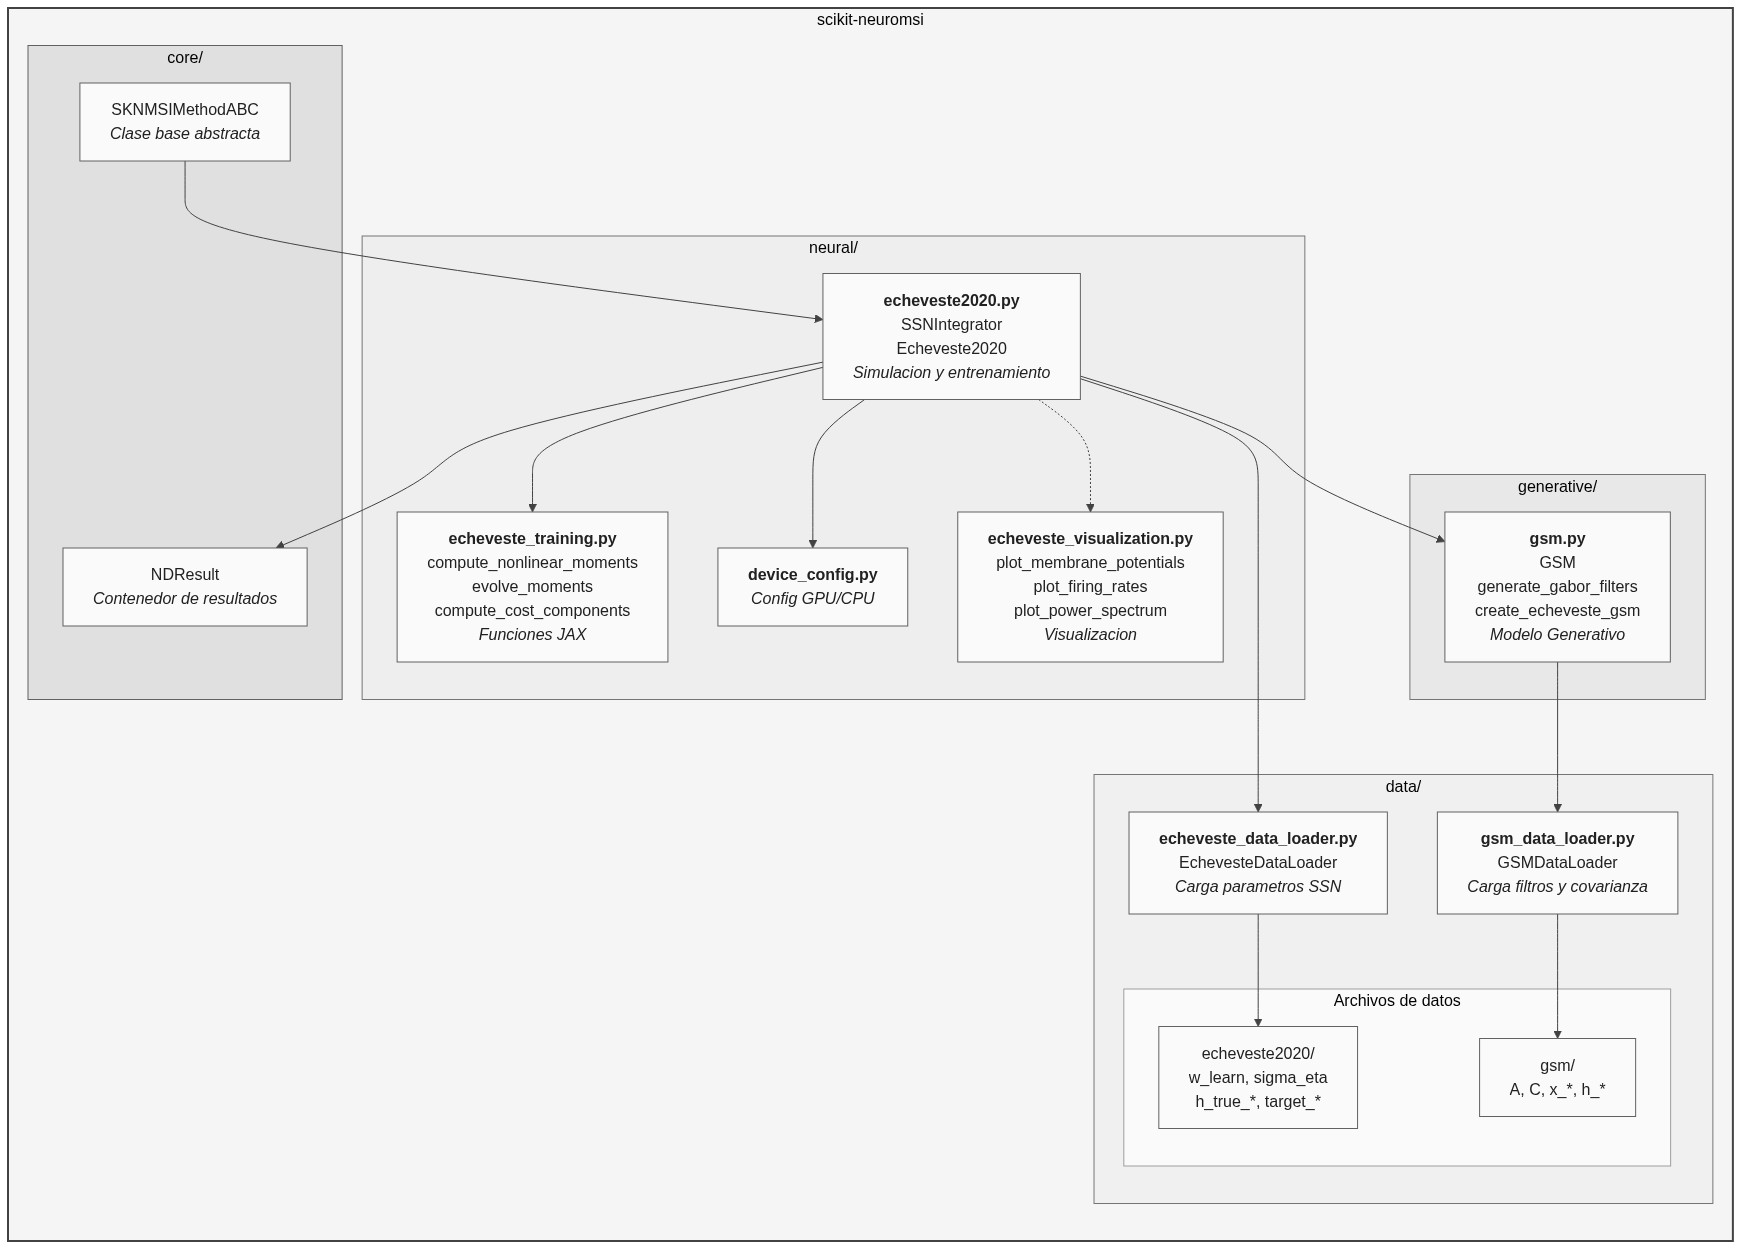
\includegraphics[width=1.3\textwidth]{10_apendice/figures/03_component_diagram_simplified.png}
    }
    \caption{
        Estructura modular del paquete scikit-neuromsi. Se detalla la organización del código en submódulos especializados: el núcleo (\texttt{core/}) con la clase base abstracta y el contenedor de resultados, el módulo neuronal (\texttt{neural/}) con las clases de simulación y las funciones de entrenamiento en JAX, el módulo generativo (\texttt{generative/}) con el modelo \acrshort{GSM}, y el sistema de gestión de datos (\texttt{data/}) con los cargadores especializados.
    }
    \label{fig:component-diagram}
\end{figure}

% --- FIGURA 2: DIAGRAMA DE CLASES ---
\begin{figure}[H]
    \centering
    \makebox[\textwidth][c]{
        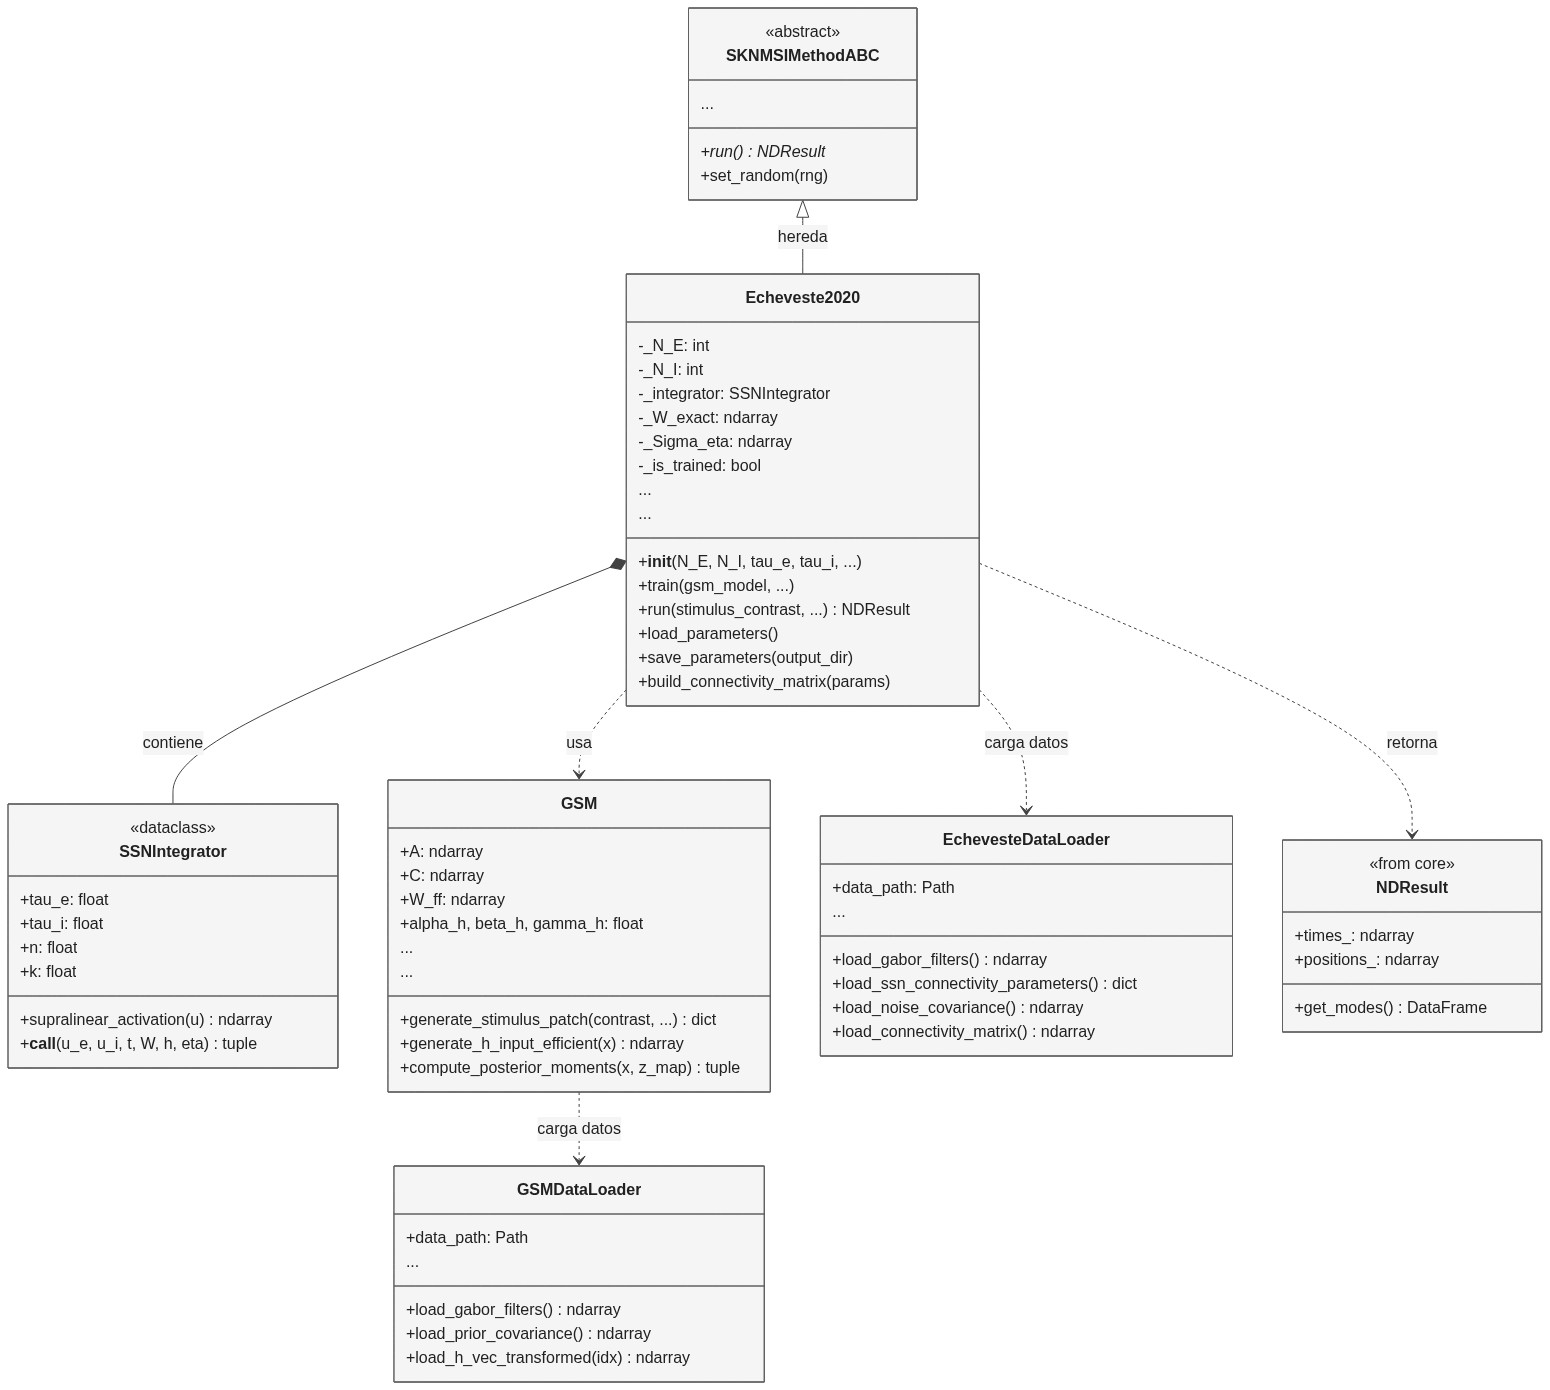
\includegraphics[width=1.3\textwidth]{10_apendice/figures/01_class_diagram_simplified.png}
    }
    \caption{
        Diagrama de clases UML detallado de la implementación Echeveste2020. Se observa la herencia desde la clase base abstracta \texttt{SKNMSIMethodABC}, la composición del integrador \texttt{SSNIntegrator} como dataclass, las dependencias con el modelo generativo \acrshort{GSM} y los cargadores de datos (\texttt{EchevesteDataLoader}, \texttt{GSMDataLoader}) para la configuración de la red. Los parámetros de los modelos están simplificados indicándolo con ``...''.
    }
    \label{fig:class-diagram}
\end{figure}

%=============================================================================
%=============================================================================

\clearpage
\newgeometry{margin=0cm}

\begin{figure}[p]
    \centering
    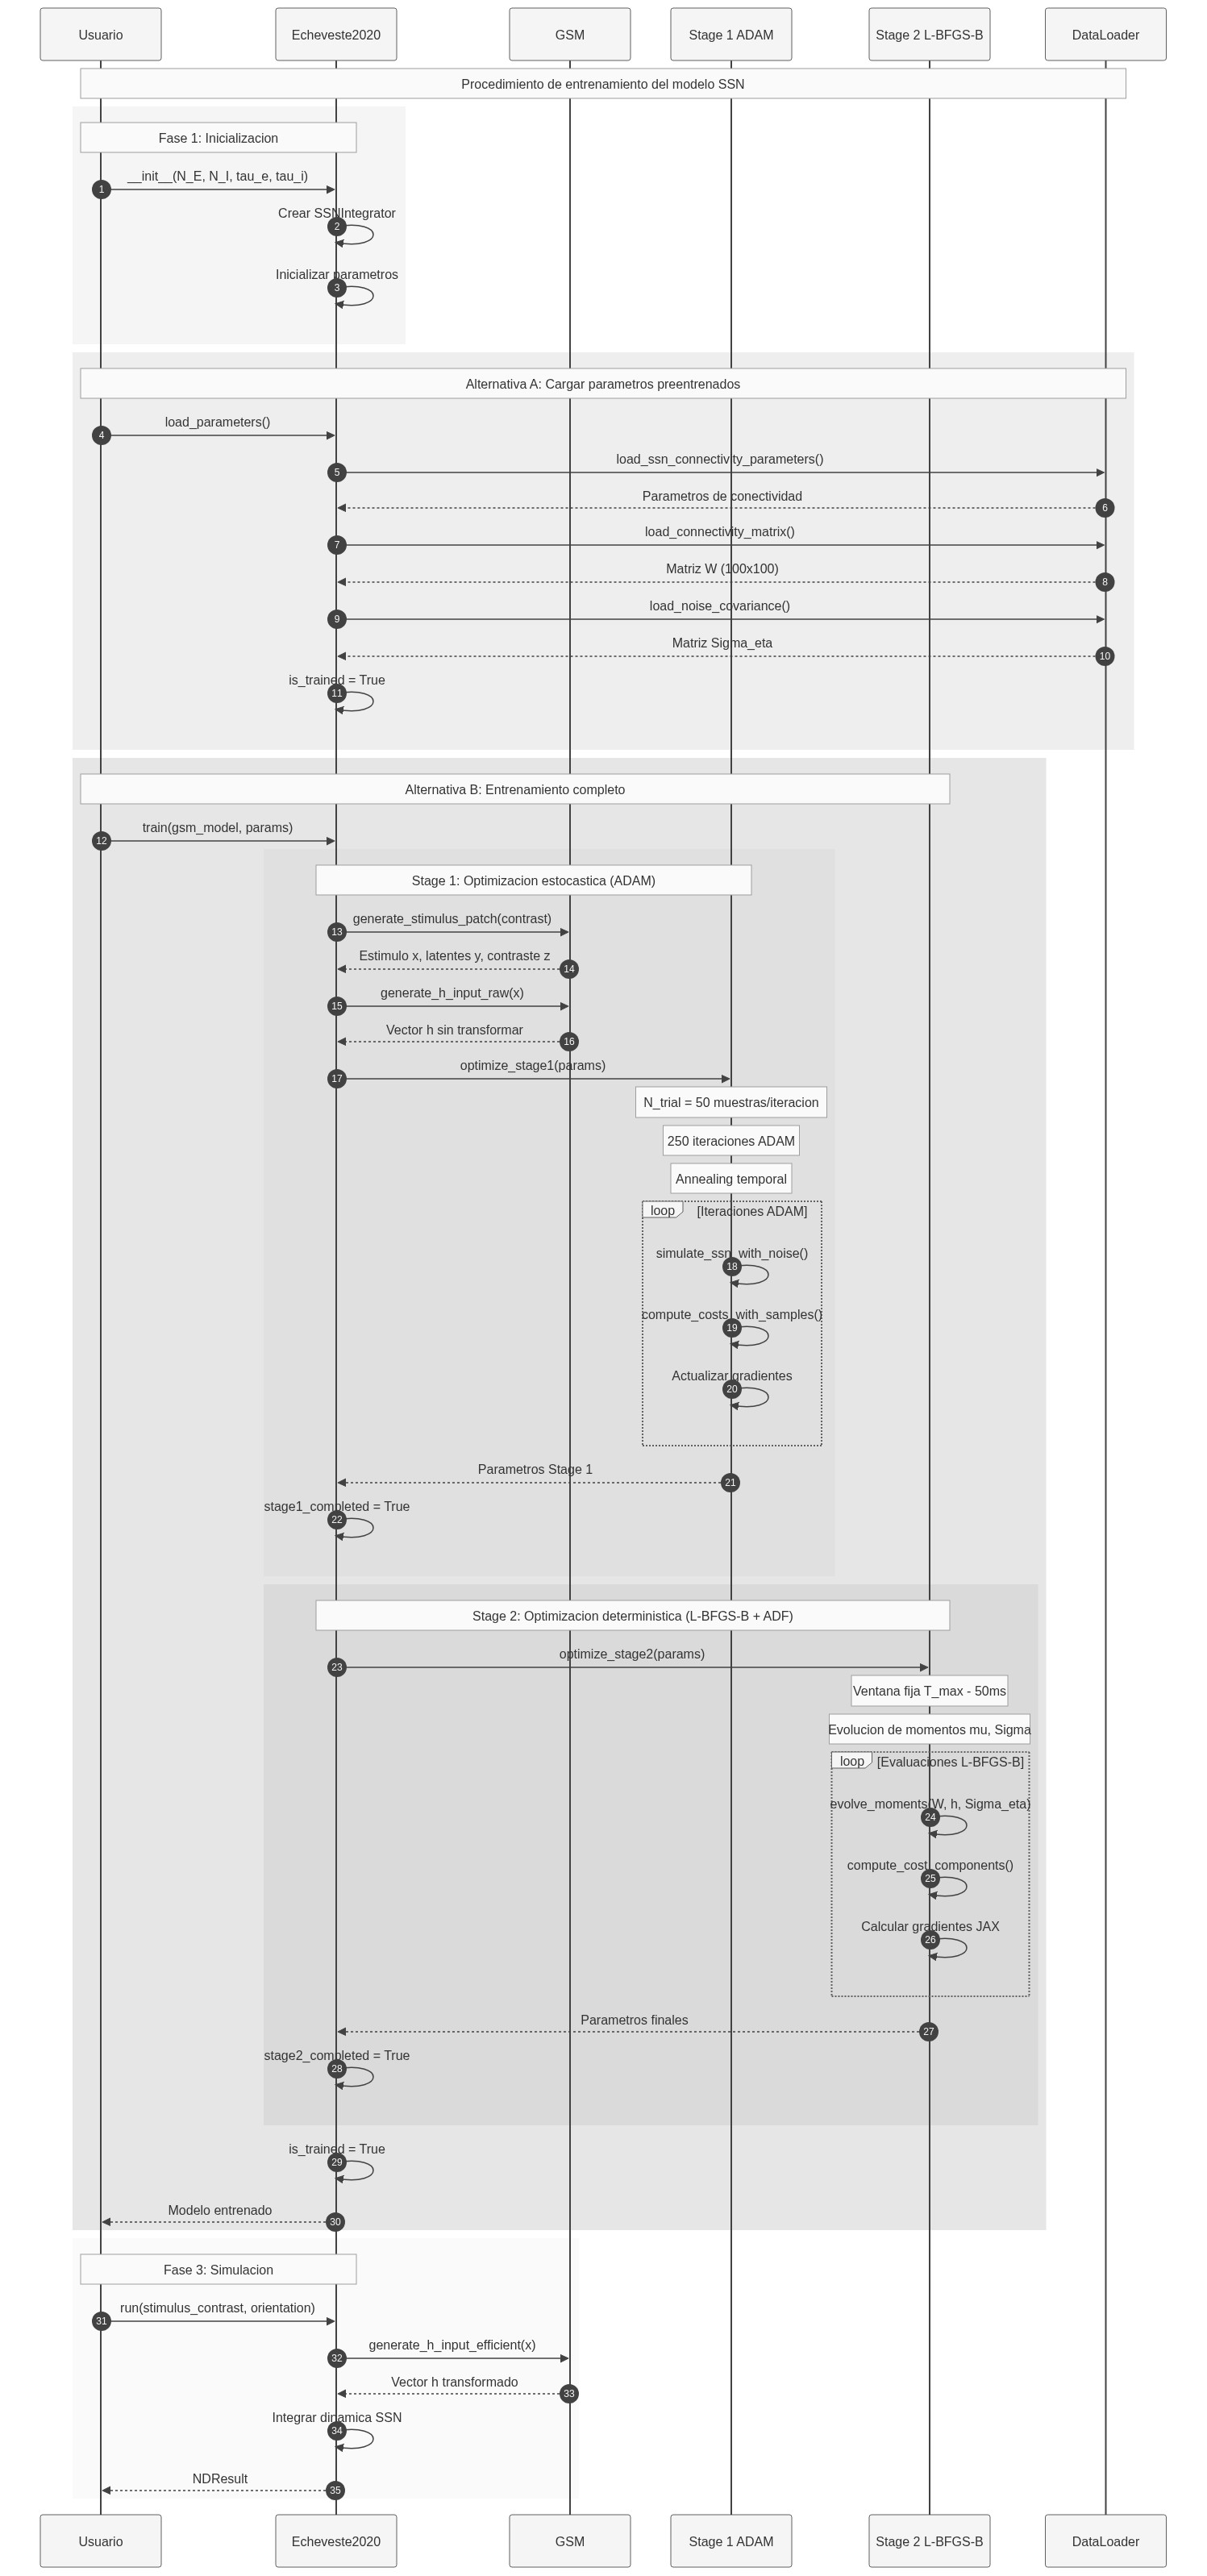
\includegraphics[width=0.9\paperwidth,height=0.8\paperheight,keepaspectratio]{10_apendice/figures/04_sequence_training_formal.png}
    \caption{Diagrama de secuencia completo del proceso de entrenamiento y validación.}
    \label{fig:sequence-training-full}
\end{figure}

\restoregeometry
\clearpage

%=============================================================================
%=============================================================================

\begin{figure}[H]
    \centering
    \makebox[\textwidth][c]{
        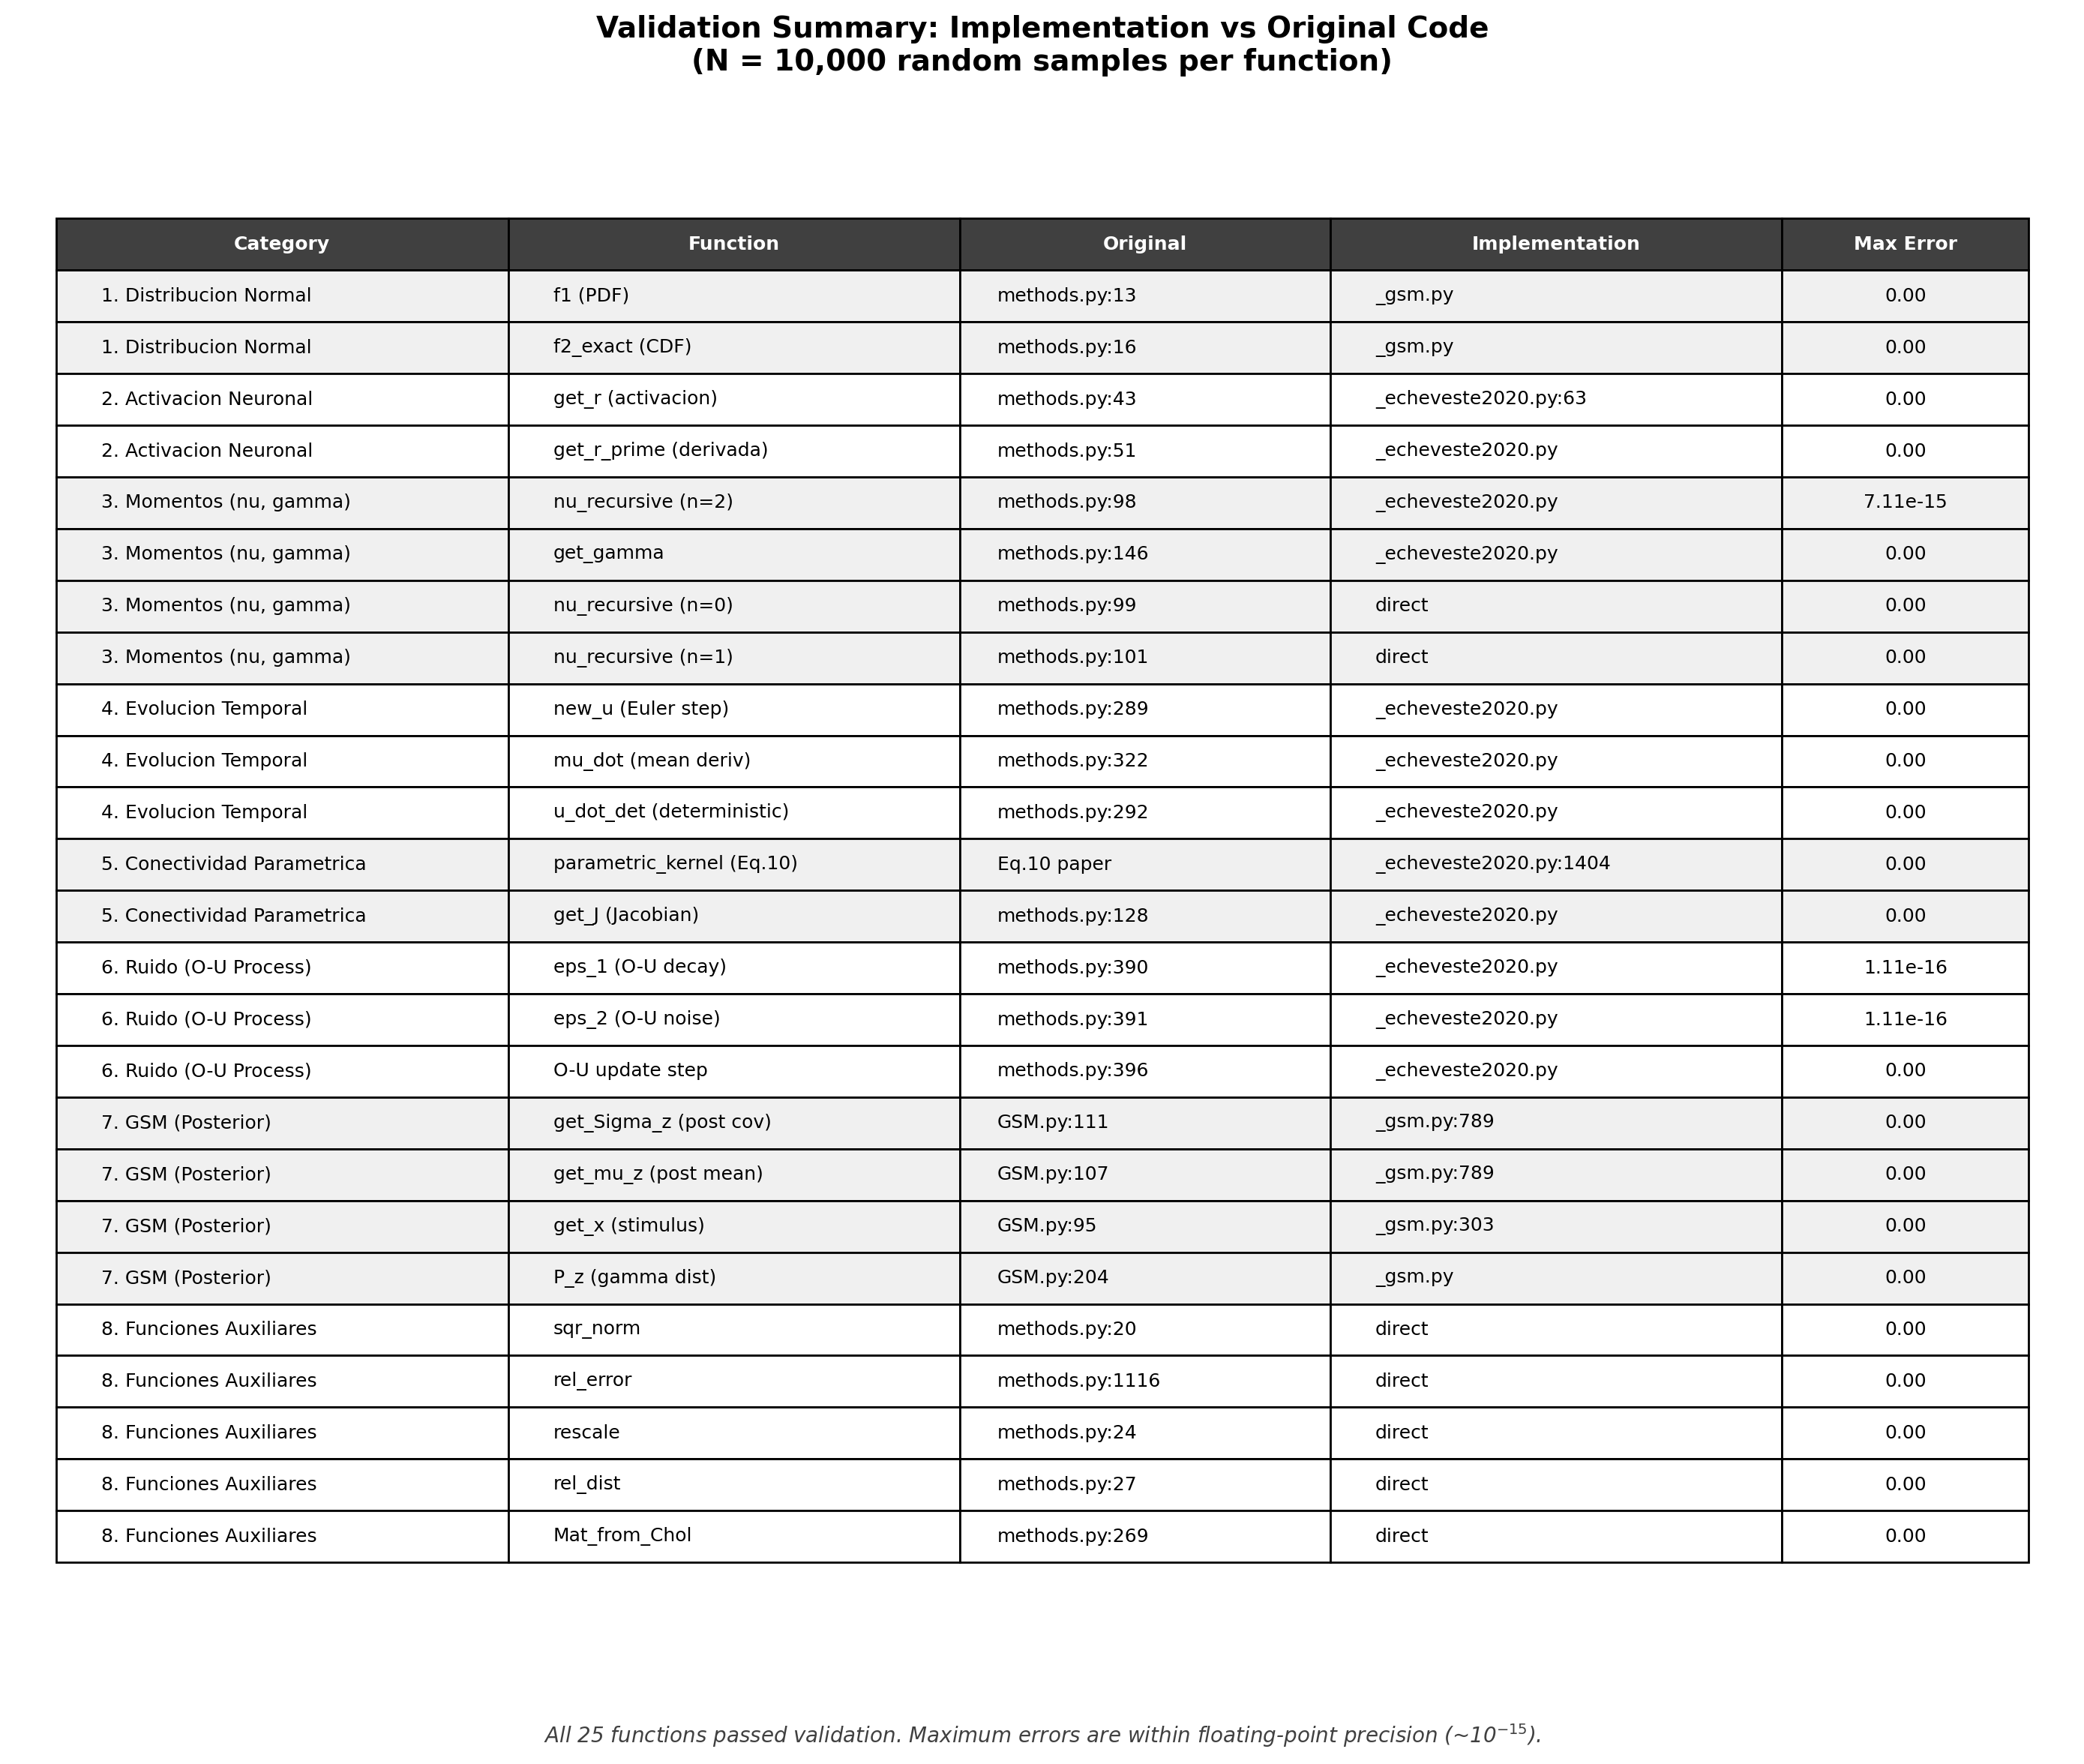
\includegraphics[width=1.3\textwidth]{10_apendice/figures/comprehensive_validation_formal.png}
    }
    \caption{
        Resumen completo de validación función por función. La tabla muestra las 25 funciones validadas, organizadas por categoría, con referencias a las líneas de código específicas tanto en el repositorio original (\texttt{methods.py}, \texttt{GSM.py}) como en nuestra implementación (\texttt{\_echeveste2020.py}, \texttt{\_gsm.py}). Todos los errores máximos están en el orden de la precisión de punto flotante ($\sim 10^{-15}$), confirmando equivalencia numérica exacta.
    }
    \label{fig:function-validation-complete}
\end{figure}
